\chapter{Introduction}
\label{section_introduction}

\singlespacing

Example document showing the features of this \LaTeX\ class. Citations are similar to any other \LaTeX\ document and require a bibtex format of the bibliography to be saved in the project directory.

\section{Figures}

Figures have to be saved in a \texttt{figures} as defined in the main \texttt{main-cu-example.tex} file. Figure \ref{fig_commercial_end_uses} shows the breakdown of commercial building energy consumption in the United States \cite{EnergyInformationAdministration2020}.

\begin{figure}[H]
	\begin{center}
		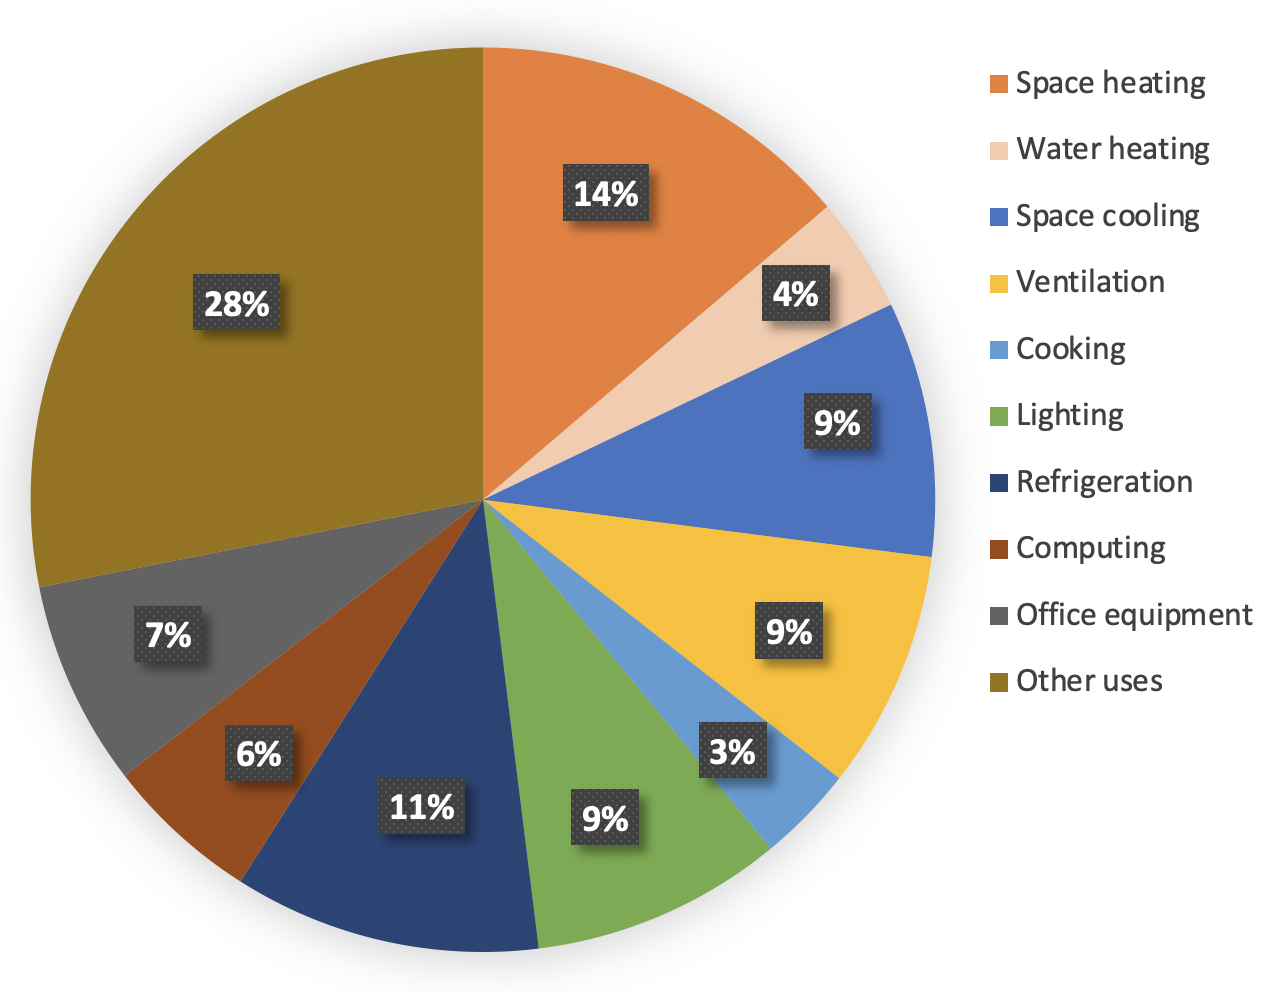
\includegraphics[width=0.5\linewidth]{fig_commercial_end_uses.png}
	\end{center}
	\caption{Commercial building energy use}
	\label{fig_commercial_end_uses}
\end{figure}

If the figure has a citation in it, then make sure to use the ``two level caption" so the citation does not appear in the table of contents. This can cause an issue when the references/citations are shown in the order of appearance. Note the use of square brackets as the first caption.

\begin{figure}[H]
	\begin{center}
		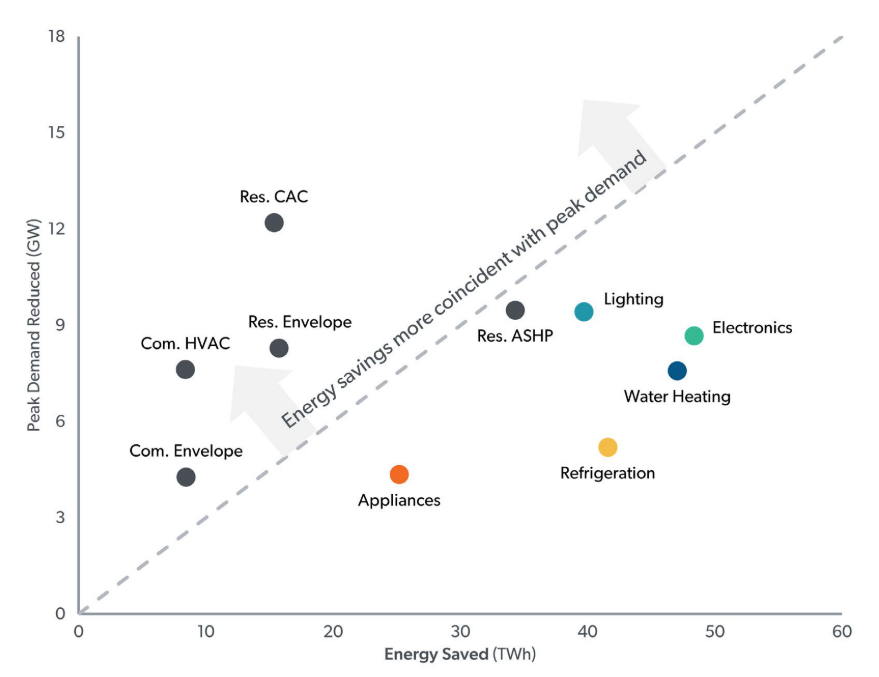
\includegraphics[width=0.5\linewidth]{fig_energy_peak_demand.png}
	\end{center}
	\caption[Peak demand reduction vs energy saved by building technology]{Peak demand reduction vs energy saved by building technology \cite{Satchwell2021}}
	\label{fig_energy_peak_demand}
\end{figure}


\section{Tables}

An example table with caption is shown in Table \ref{tbl_example}.

\begin{table}[H]
	\centering
	\caption{Example table of objectives}
	\begin{tabular}{|L{4.5cm}|L{5.5cm}|L{5.0cm}|}
		\hline
		\rowcolor{lightgray}
		\textbf{Research Objective}                                                                                                                       & \textbf{Method of Achievement} & \textbf{Expected Outcome} \\ \hline \hline
		% next row
		Cell 1                                                                                                                                            & Cell 2                         & Cell 2                    \\ \hline
		% next row
		Another cell                                                                                                                                      &
		And another cell with some text wrapping if there is enough text needed for it to wrap based on the fixed width defined in the tabular definition &
		Last cell for this row                                                                                                                                                                                         \\ \hline
	\end{tabular}
	\label{tbl_example}
\end{table}

\section{Equations}

ASHRAE Guideline 14's \cite{Landsberg2014} \gls{CVRMSE} and \gls{NMBE} calculations shown in Equations \ref{eq_cvrmse} and \ref{eq_nmbe}, respectively, as well as $r^2$ and various visual plots generated by the \gls{MMF}.

\begin{equation}
	\label{eq_cvrmse}
	CVRMSE=\frac{1}{\bar{y}}\sqrt{\frac{\sum{(y_i-\hat{y}_i)^2}}{n-1}}
\end{equation}
where $y_i$ is the actual data at timestep, $i$, $\hat{y}_i$ is the modeled (or estimate) of the data at timestep, $i$, $\bar{y}$ is the mean of the actual data, and $n$ is the number of samples.

\bigskip

\begin{equation}
	\label{eq_nmbe}
	NMBE=\frac{\sum{(y_i - \hat{y}_i})}{(n-1) \cdot \bar{y}}
\end{equation}
where $y_i$ is the actual data at timestep, $i$, $\hat{y}_i$ is the modeled (or estimate) of the data at timestep, $i$, $\bar{y}$ is the mean of the actual data, and $n$ is the number of samples.


\section{Acronyms}

This document also demonstrates the use of a glossary to provide acronym definitions. The definitions are stores in the \texttt{acronyms.tex} file. For example, a \gls{DES} will be fully defined the first time, then after \gls{DES} will be an acronym. This is a nice feature because if text moves then \LaTeX\ will handle when to spell out the acronym first. The glossary also allows for pluralization, for example \glspl{GEB} will be defined as plural, but later uses can still be singular. A \gls{GEB} is already defined. Lastly, if the acronym glossary contains more items than defined in the document, it will only show the ones that are used.

Note that this functionality is not visible in the PDF that is produced attached to the GitHub action. To run this functionality, your \LaTeX\ environment needs to build the glossary first. In TexStudio this is done by adding \texttt{txs:///makeglossaries} to your build setting. On Overleaf, this works out of the box.

\section{Lists and Enumerations}

Example of nested enumeration and lists (also known as itemize in \LaTeX\ speak).

\begin{enumerate}
	\item First item
	      \begin{itemize}
		      \item Example of just a bullet item
		      \item Another item
		      \item Last item!
	      \end{itemize}

	\item Second numbered item
	      \begin{enumerate}
		      \item Keep the list going,
		      \item With more items,
		      \item But now I'm done.
	      \end{enumerate}
\end{enumerate}

\section{Code Snippets}

An example of code snippets is shown in Python Code \ref{code_gmt_python} below. The code can be used to generate the updated Modelica source code in Code \ref{code_gmt_modelica}.

\begin{lstlisting}[language=Python, backgroundcolor=\color{aliceblue}, caption={Python snippets of Modelica Builder commands}, captionpos=b, label={code_gmt_python}]
	mofile.rename_component_argument(
		"Buildings.ThermalZones.ReducedOrder.EquivalentAirTemperature.VDI6007",
		"eqAirTempVDI",
		"hConvWallOut",
		"hConWallOut"
	)
	
	mofile.add_connect(
		'port_a', f'{thermal_zone_name}.intGainsConv',
		annotations=['Line(points={{0,100},{96,100},{96,20},{92,20}}, color={191,0,0})']
	)
	
	mofile.add_connect(
		f'{thermal_zone_name}.TAir', 'TAir',
		annotations=[
			'Line(points={{93,32},{98,32},{98,48},{110,48}}, color={0,0,127})'
		]
	)
\end{lstlisting}

% Add in a bigskip between code snippets
\bigskip

\begin{lstlisting}[language=Modelica, backgroundcolor=\color{aliceblue}, caption={Updated Modelica code after Modelica Builder}, captionpos=b, label={code_gmt_modelica}]
	Buildings.ThermalZones.ReducedOrder.EquivalentAirTemperature.VDI6007 eqAirTempVDI(
		aExt=0.5,
		wfGro=0,
		hConWallOut=20.0,
		hRad=5.0,
		n=1,
		wfWall={1.0},
		wfWin={0},
		TGro=285.15) "Computes equivalent air temperature for roof"
		annotation (Placement(transformation(extent={{30,34},{50,54}})));
	
	// ... 
	
	connect(personsConv.port, thermalZoneFourElements.intGainsConv)
		annotation (
			Line(points={{68,-52},{96,-52},{96,20},{92,20}}, color={191,0,0}));
	
	connect(thermalZoneFourElements.TAir, TAir) 
		annotation(
			Line(points={{93,32},{98,32},{98,48},{110,48}}, color={0,0,127}));		
\end{lstlisting}



